\documentclass[10pt]{article}
\usepackage[usenames]{color} %used for font color
\usepackage{amssymb} %maths
\usepackage{amsmath} %maths
\usepackage[utf8]{inputenc} %useful to type directly diacritic characters
\usepackage{tikz}
\usetikzlibrary{arrows,positioning,decorations.pathreplacing}

\definecolor{boiseBlue} {RGB}{29,72,159}
\definecolor{rojoAmor} {RGB}{171,13,4}
\definecolor{moradoAmor} {RGB}{93,8,113}
\definecolor{verdeAmor} {RGB}{98,158,31}
\definecolor{negro} {RGB}{10,10,10}
\definecolor{lgreen} {RGB}{180,210,100}
\definecolor{dblue}  {RGB}{20,66,129}
\definecolor{ddblue} {RGB}{11,36,69}
\definecolor{lred}   {RGB}{220,0,0}
\definecolor{nred}   {RGB}{224,0,0}
\definecolor{norange}{RGB}{230,120,20}
\definecolor{nyellow}{RGB}{255,221,0}
\definecolor{ngreen} {RGB}{98,158,31}
\definecolor{dgreen} {RGB}{78,138,21}
\definecolor{nblue}  {RGB}{28,130,185}
\definecolor{jblue}  {RGB}{20,50,100}\begin{document}
\[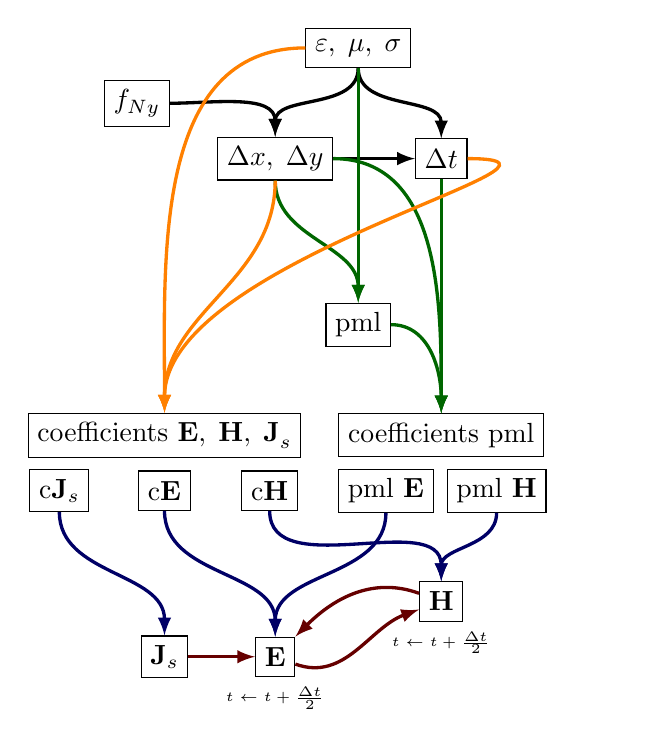
\begin{tikzpicture}[>=latex]
%
\node[rectangle,draw,minimum size=0.5cm] at (0,0)  (p) {$\varepsilon,\;\mu,\;\sigma$};
\node[rectangle,draw,minimum size=0.5cm] at (-8em,-2em)  (f) {$f_{Ny}$};
\node[rectangle,draw,minimum size=0.5cm] at (-3em,-4em)  (dxdy) {$\Delta x,\;\Delta y$};
\node[rectangle,draw,minimum size=0.5cm] at (3em,-4em)  (dt) {$\Delta t$};
\node[rectangle,draw,minimum size=0.5cm] at (0,-10em)  (pml) {pml};
\node[rectangle,draw,minimum size=0.5cm] at (3em,-14em)  (cpml) {coefficients pml};
\node[rectangle,draw,minimum size=0.5cm] at (1em,-16em)  (pmlE) {pml ${\bf E}$};
\node[rectangle,draw,minimum size=0.5cm] at (5em,-16em)  (pmlH) {pml ${\bf H}$};
\node[rectangle,draw,minimum size=0.5cm] at (-7em,-14em)  (cEHJ) {coefficients ${\bf E,\; H,\; J}_s$};
\node[rectangle,draw,minimum size=0.5cm] at (-10.8em,-16em)  (cJ) {c${\bf J}_s$};
\node[rectangle,draw,minimum size=0.5cm] at (-7em,-16em)  (cE) {c${\bf E}$};
\node[rectangle,draw,minimum size=0.5cm] at (-3.2em,-16em)  (cH) {c${\bf H}$};
%
\node[rectangle,draw,minimum size=0.5cm] at (3em,-20em)  (H) {${\bf H}$};
\node[minimum size=0.5cm] at (3em,-21.5em)  () {\tiny{$t\leftarrow t+\frac{\Delta t}{2}$}};
\node[rectangle,draw,minimum size=0.5cm] at (-3em,-22em)  (E) {${\bf E}$};
\node[minimum size=0.5cm] at (-3em,-23.5em)  () {\tiny{$t\leftarrow t+\frac{\Delta t}{2}$}};
\node[rectangle,draw,minimum size=0.5cm] at (-7em,-22em)  (J) {${\bf J}_s$};
%
\draw[->,very thick,black]
  (p) to[out=270,in=90] (dxdy);
\draw[->,very thick,black]
  (f) to[out=0,in=90] (dxdy);
\draw[->,very thick,black]
  (p) to[out=270,in=90] (dt);
\draw[->,very thick,black]
  (dxdy) to[out=0,in=180] (dt);
\draw[->,very thick,black!60!green]
  (p) to[out=270,in=90] (pml);
\draw[->,very thick,black!60!green]
  (dxdy) to[out=270,in=90] (pml);
\draw[->,very thick,black!60!green]
  (pml) to[out=0,in=90] (cpml);
\draw[->,very thick,black!60!green]
  (dt) to[out=270,in=90] (cpml);
\draw[->,very thick,black!60!green]
  (dxdy) to[out=0,in=90] (cpml);
\draw[->,very thick,orange]
  (dxdy) to[out=270,in=90] (cEHJ);
\draw[->,very thick,orange]
  (p) to[out=180,in=90] (cEHJ);
\draw[->,very thick,orange]
  (dt) to[out=0,in=90] (cEHJ);
%
\draw[->,very thick,black!60!blue]
  (pmlH) to[out=270,in=90] (H);
\draw[->,very thick,black!60!blue]
  (cH) to[out=270,in=90] (H);
\draw[->,very thick,black!60!blue]
  (cE) to[out=270,in=90] (E);
\draw[->,very thick,black!60!blue]
  (pmlE) to[out=270,in=90] (E);
\draw[->,very thick,black!60!blue]
  (cJ) to[out=270,in=90] (J);
\draw[->,very thick,black!60!red]
  (J) to[out=0,in=180] (E);
\draw[->,very thick,black!60!red]
  (H) to[out=160,in=45] (E);
\draw[->,very thick,black!60!red]
  (E) to[out=-20,in=200] (H);
%
\end{tikzpicture}
\]
\end{document}